% Chapter 7: The Stabilisers
% Complete rewrite 2025-12-08: biological explanatory style throughout

\chapter{The Stabilisers}
\label{ch:stabilisers}

\epigraph{The general rule would establish itself insensibly, and by slow degrees, in consequence of that love of analogy and similarity of sound, which is the foundation of by far the greater part of the rules of grammar.}{Adam Smith, \textit{Considerations Concerning the First Formation of Languages} (1761)}

When a biologist asks what a macrophage is, they don't look for a definition; they look for properties that tend to co-occur: typical functions (phagocytosis, antigen presentation), marker profiles, developmental origins. None is strictly necessary~-- some macrophages don't phagocytose; some share markers with dendritic cells~-- but because the properties cluster reliably, the category supports prediction and experimental design. The parallel is methodological, not ontological: I'm borrowing an explanatory style, not claiming that grammars are organisms.

Adam Smith saw something similar in grammar two and a half centuries ago. Rules \enquote{establish themselves insensibly, and by slow degrees}~-- not by fiat, but through the accumulated pressure of analogy and pattern-matching. This chapter adds the causal machinery that makes that slow consolidation intelligible. What keeps grammatical categories stable?


\section{The cluster}
\label{sec:7:the-cluster}

The cluster-first strategy applies to grammar directly. The same approach that lets immunologists sidestep definitional impasses can do the same for linguists.

Take nouns. In English, items we call nouns typically take determiners (\mention{the dog}, \mention{a problem}), inflect for number (\mention{dogs}, \mention{problems}), function as heads of noun phrases in subject and object positions, refer to entities or entity-like abstractions, and are commonly modified by adjectives. None of these is strictly necessary: \mention{cattle} lacks a singular; names resist determiners; \mention{information} doesn't pluralise. Cross-linguistically, the picture is messier still: Mandarin nouns don't inflect for number at all. And yet typologists recognise something noun-like across systems.

This is the position the chapter defends: grammatical categories are mechanism-maintained kinds whose reality is indexed to inductive utility, not definitional necessity~-- stabilised by a braid of cognitive, social, and physical processes. The clustering they produce is stable enough, cross-contextually robust enough, that predictions based on category membership reliably succeed.

The question is no longer: what is the essence of noun-ness? Although linguists tried that approach~-- across semantic, distributional, and morphosyntactic definitions~-- it generated boundary disputes and competing proposals but no stable resolution. The mechanism-first question is different: what keeps the cluster clustered~-- what does the stabilising work?

Grammatical categories are neither fully mind-independent natural kinds~-- like chemical elements~-- nor purely conventional human kinds that exist only because we agree they do, like money or traffic laws. They are a third thing: real enough to support induction, socially embedded enough to change under pressure. They lack the essences that define elements, but they resist the arbitrary revision that conventions permit.

\enquote{Mechanism} in this book means something specific: a mechanism posit earns its keep by specifying component processes whose interactions produce the target phenomenon. If you can't say what sub-processes combine to yield the clustering and what would happen if one were disrupted, you don't yet have a mechanism~-- you have a label with causal pretensions. Labelling a pile of bricks \enquote{Wall} does not make it load-bearing; only stabilising processes do. In molecular biology, mechanisms are crisply bounded: the ribosome, the spliceosome, the gene regulatory network. For grammatical categories, the stabilisers are less crisply bounded~-- they include processing biases, acquisition pathways, social indexing, transmission dynamics~-- but the constraint is the same: the term is elastic enough to span cognitive and social scales, yet not so elastic that any correlation gets to call itself mechanistic.

\term{Stabiliser} is a related term. Where \enquote{mechanism} emphasises causal structure, \enquote{stabiliser} emphasises the functional role~-- what keeps the cluster clustered. A stabiliser is a mechanism insofar as it has causal depth, but the term foregrounds maintenance rather than mere causation. Something counts as a stabiliser if removing it would change the clustering~-- if the category would fragment, drift, or dissolve. A mere correlate~-- something that co-occurs with the category but doesn't contribute to its maintenance, like the orthographic length of a word that happens to be a noun~-- is not a stabiliser.





\section{Stabilisers at multiple scales}
\label{sec:7:stabilisers-at-scales}

What the biological template provides is visibility: it lets us see variation as activation rather than noise, boundaries as dynamic rather than definitional, and stability as achieved rather than given. Without this framing, gradient membership looks like failed classification; with it, gradient membership becomes evidence about which mechanisms are operating and where.

The analogy is not homology. Cell biologists ask what mechanisms maintain the macrophage phenotype; we ask what mechanisms maintain the noun category. The question structure is the same; the mechanisms themselves are domain-specific. The parallel earns its keep by making linguistic phenomena more visible and testable.

\begin{table}[htbp]
\centering
\small
\begin{tabular}{@{}p{2.8cm}p{5.5cm}p{5.5cm}@{}}
\toprule
\textbf{Scale} & \textbf{Biology} & \textbf{Linguistics} \\
\midrule
Dynamical basins & \textbf{Gene regulatory networks} produce attractor states~-- stable configurations the cell tends to settle into and return to when perturbed. The basins are emergent from ongoing interaction and exist only as long as stabilising processes continue. & \textbf{Cognitive architectures and processing biases} produce attractor states. A construction frequent enough becomes entrenched~-- produced as a unit rather than assembled. This is dynamical, not definitional. \\
\addlinespace
Developmental trajectory & \textbf{Developmental lineage} constrains which basins are reachable. A cell's history matters: what precursors it passed through, what signals it received at critical windows. & \textbf{Acquisition pathways and learning biases} constrain what a speaker can learn. Order of acquisition matters. Early-learned patterns anchor later ones. Sensitive phases exist where input has disproportionate effect. \\
\addlinespace
Microenvironmental modulation & \textbf{Microenvironmental signalling}~-- local cytokines, tissue context~-- pushes cells into different regions of the same basin, producing variation within the type. & \textbf{Discourse context and pragmatic ecology} push tokens into different regions of the distributional space. Same category, different activation state. Variation is expected, not noise. \\
\addlinespace
Reciprocal feedback & \textbf{Functional feedback}: what the cell does alters its microenvironment, which sustains or shifts its state. The stabilisation is not one-way. & \textbf{Functional feedback}: what speakers do with categories alters input to the next generation, which alters what categories stabilise. Usage facilitates reconstruction; facilitated patterns shape usage. \\
\bottomrule
\end{tabular}
\caption{Multi-level stabilisation: biology and linguistics in parallel.}
\label{tab:stabiliser-parallel}
\end{table}

Table~\ref{tab:stabiliser-parallel} traces kinds of stabilising stories; Figure~\ref{fig:mechanism-typology} reorganises the same mechanisms by timescale and locus, which determines what evidence is relevant. Claims about fast mechanisms (Quadrants I--II) require online processing measures; claims about slow mechanisms (Quadrants III--IV) require longitudinal and apparent-time data.

\begin{figure}[htbp]
\centering
\begin{tikzpicture}[
    quadrant/.style={minimum width=4.5cm, minimum height=3cm, align=center, font=\small},
    axislabel/.style={font=\small\bfseries},
    mechanism/.style={font=\small},
    sublabel/.style={font=\scriptsize, text=black!70}
]

% Quadrant backgrounds
\fill[black!5] (-4.5, 0) rectangle (0, 3);
\fill[black!12] (0, 0) rectangle (4.5, 3);
\fill[black!12] (-4.5, -3) rectangle (0, 0);
\fill[black!5] (0, -3) rectangle (4.5, 0);

% Axes
\draw[thick, -{Stealth[length=3mm]}] (-4.8, 0) -- (5, 0);
\draw[thick, -{Stealth[length=3mm]}] (0, -3.3) -- (0, 3.5);

% Axis labels
\node[axislabel, left] at (-4.8, 0) {Individual};
\node[axislabel, right] at (5, 0) {Community};
\node[axislabel, above, align=center] at (0, 3.5) {Fast\\[-2pt]{\scriptsize\color{black!70}(ms--minutes)}};
\node[axislabel, below, align=center] at (0, -3.3) {Slow\\[-2pt]{\scriptsize\color{black!70}(months--generations)}};

% Quadrant contents
% Top-left: Fast + Individual
\node[mechanism, align=center] at (-2.25, 1.5) {Processing economy\\[4pt]Predictive facilitation};

% Top-right: Fast + Community
\node[mechanism, align=center] at (2.25, 1.5) {Accommodation\\[4pt]Alignment in dialogue};

% Bottom-left: Slow + Individual
\node[mechanism, align=center] at (-2.25, -1.5) {Acquisition\\[4pt]Entrenchment};

% Bottom-right: Slow + Community
\node[mechanism, align=center] at (2.25, -1.5) {Transmission dynamics\\[4pt]Social indexing};

% Quadrant labels (optional, subtle)
\node[sublabel] at (-4, 2.6) {I};
\node[sublabel] at (4, 2.6) {II};
\node[sublabel] at (-4, -2.6) {III};
\node[sublabel] at (4, -2.6) {IV};

\end{tikzpicture}
\caption{Mechanism typology by timescale and locus.}
\label{fig:mechanism-typology}
\end{figure}

The definition tells you what the cluster looks like at a moment. The stabilising story tells you why it persists.

The four-level story is a heuristic, not a template. Different categories are maintained by different braids of mechanisms; the exact mapping varies. Quotatives, as we'll see, involve processing economy, social indexing, and transmission dynamics~-- mechanisms that cross-cut the four levels rather than mapping onto them one-to-one. The point is multi-level stabilisation, not exact correspondence. What the biological parallel provides is a style of explanation~-- look for mechanisms at multiple timescales, expect reciprocal feedback~-- not a fixed inventory. The case studies that follow apply this style to two deliberately different phenomena: quotatives (socially vivid, spreading through youth networks) and filler-gap constructions (more syntactic, depending on information structure). If the framework earns explanatory traction for both, it's not just sociolinguistics with a new label.


\section{Variation as activation states}
\label{sec:7:variation-activation-states}

The immunologist's key move: variation within a category is not embarrassing fuzziness to be explained away. It's the expected signature of a kind that is maintained by context-sensitive mechanisms.

A macrophage in inflamed tissue shows different markers than a macrophage in healthy tissue, but both are macrophages. The difference is activation state~-- which signals the cell has received, which region of the phenotypic space it currently occupies. The category is real, and so is the variation; both are explained by the stabilising dynamics. The same logic applies to linguistic categories.

Two kinds of variation matter, and the distinction is stabiliser-relevant. Some apparent boundary cases are \emph{within-speaker} shifts~-- the same person producing different patterns in different contexts. These are activation-state differences: one grammar, multiple accessible patterns. Others are \emph{between-speaker} differences~-- not everyone has entrenched the same patterns to the same depth. Speakers with different input histories, different literacy experiences, different interactional ecologies end up with different category boundaries. Within-speaker variation shows that categories are context-sensitive; between-speaker variation shows that they are experience-dependent. Both are part of the data that a theory of category maintenance needs to explain.

That in turn distinguishes \emph{exposure-dependent stabilisation} from \emph{population-wide stabilisation}. A category that stabilises only in speakers with particular exposure profiles is a different kind from one that stabilises across the population. The former is maintained by mechanisms that not everyone encounters; the latter is maintained by mechanisms that operate across the population.

Consider \mention{fast}. Traditional grammars call it an adjective in \mention{a fast car} (attributive modifier position) and an adverb in \mention{she ran fast} (post-verbal modifier, no \mention{-ly} suffix). Same lexeme, different syntactic behaviour. The question ``is \mention{fast} an adjective or an adverb?'' assumes a forced choice. Three frameworks give different answers.

The essentialist answer: it must be one or the other, or else homonymous (two lexemes, same form). The prototype answer: it's a gradient case, partly adjective, partly adverb, with no fact of the matter about which it ``really'' is.

The maintenance answer is different. \mention{Fast} sits on a plateau linked to both the adjectival and adverbial basins~-- a region where both diagnostic profiles remain accessible (see Figure~\ref{fig:basin-visualization}). The lexeme is stable; what varies is the token's route, determined by syntactic frame. Attributive position takes the adjectival pass (comparison, agreement in languages that have it); post-verbal position takes the adverbial one. That's stability at the type level with choice at the token level~-- not a new essence, but terrain that permits dual access.

The same framing applies to aspect in Polish. As §\ref{sec:6:mechanistic-alternative} showed, 90\% of verbs strongly prefer one aspect~-- they're deep in a single basin. The remaining verbs occupy shallower regions where contextual signals matter more. The verbs that require explicit contextual cues to disambiguate are the ones where entrenchment is weaker, where the tense-frame signal has more work to do. That's the activation-state picture applied to grammatical aspect. Section~\ref{sec:7:filler-gap-whose} applies the same idea to a construction rather than a lexeme: independent relative \mention{whose}, which succeeds under specific licensing conditions and fails without them.

The activation-state logic has neural consequences. If categories are maintained by interacting cues rather than definitions, then processing should track graded predictive fit, not all-or-none membership. Event-related potentials offer a window here, though the picture is messier than textbook summaries suggest. Components like the N400 and P600 don't map cleanly onto `semantic' versus `syntactic' violations; their amplitude and timing reflect prediction error and retrieval difficulty in ways that cut across traditional module boundaries. What matters for the present argument is the pattern: HPC predicts continuous sensitivity to cue convergence~-- the more cues align, the stronger the facilitation; the more they conflict, the larger the processing cost. Classical definitional categories predict bimodal profiles~-- clear members and clear non-members~-- with borderline cases showing high variance rather than intermediate values. Under HPC, borderline items should show systematic intermediate values: graded neural profiles that track cue-weighting, not random scatter around a binary threshold. That's a testable contrast.



\section{One case in depth: the emergence of new quotatives}
\label{sec:7:one-case}

Rather than enumerate mechanisms abstractly, let's trace the stabilising story for one category: the quotative marker.

Quotatives introduce reported speech, thought, gesture, or sound. The functional need to distinguish the narrator's voice from the character's is presumably as old as narrative itself. But when we look across typologically unrelated languages, we find a striking convergence in recent history: in the late twentieth century, new quotative forms emerged or expanded~-- forms with a distinctive profile that spread through similar populations and stabilised through similar mechanisms.

The English case is well documented, and the chronology reveals the dynamical logic: what emerges first, what locks in later, and which contexts serve as incubators.

\textcite{butters1982} first noted \mention{be like} in American English in 1982, observing its use to report unuttered thoughts: \mention{I was like, `Let me live, Lord'}. \textcite{ferrarabell1995} hypothesised that the form originated with first-person subjects and internal dialogue before expanding to third-person subjects and direct speech. The incubator was informal peer narrative~-- storytelling among friends, where enactment matters more than accuracy. By the mid-1990s, the form had spread beyond that niche. \textcite{tagliamontedarcy2004} tracked apparent-time data from Canadian English: in 1995, speakers aged 18--27 used \mention{be like} for 13\% of quotative tokens; by 2003, speakers aged 17--19 used it for 63\%~-- a fivefold increase in under a decade. The same cohort, re-sampled seven years later, showed \mention{be like} rising from 13\% to 31\% as they aged into their thirties \autocite{tagliamontedarcy2007}. This is not age-grading; it's real-time change, with each generation carrying its quotative inventory into adulthood. What began as a micro-regularity in peer narrative became a meso-level entrenchment in a generation's speech, and then a macro-level category expectation that shapes input to the next generation.

German shows a parallel trajectory. \textcite{golato2000} analysed \mention{und ich so} (`and I'm like') in video-recorded conversations, documenting its function in storytelling: introducing punchlines, sound effects, gestures, and verbal enactments~-- the same profile as English \mention{be like}. The form was attested in youth speech by the late 1990s \autocite{androutsopoulos1998} and has since become established among younger German speakers, though it remains more register-restricted than its English counterpart.

Japanese \mention{tte} (reduced from \mention{to itte}, `saying that') functions similarly: a phonologically light form that introduces reported speech, thought, or stance in informal narrative. The pattern extends to Turkish \mention{diye} (converb of \mention{demek}, `to say'), which has expanded from its older quotative functions into increasingly colloquial discourse contexts.

\textcite{buchstaller2014} synthesises the cross-linguistic evidence: the emergence of these innovative quotatives reflects independent development under similar functional pressures, rather than media-driven borrowing. Different sources, different structures, same functional niche, same stabilising dynamics.

This is not coincidence, but convergent maintenance: independent forms, stabilised by the same mechanisms, producing the same category architecture.

\subsection{The quotative cluster}

What properties co-occur in these new quotatives? The distributional studies reveal a consistent profile.

\textbf{Non-lexical content.} These forms introduce material that goes beyond words: gesture, facial expression, tone of voice, inner monologue. \mention{And I was like} doesn't just report what someone said; it enacts the experience---recruiting prosody, embodied performance, and affective display as part of the quotation. \textcite{ferrarabell1995} noted that early \mention{be like} tokens disproportionately introduced internal states and non-lexicalised sounds~-- groans, sighs, exclamations~-- before expanding to verbatim-style direct speech. \textcite{golato2000} documented the same pattern for German \mention{so}: it turns reported speech into performance.

\textbf{First-person and present-tense preference.} The forms attach preferentially to first-person subjects and historical-present tense. \textcite{tagliamontedarcy2004} found that in their Toronto data, first-person contexts strongly favoured \mention{be like} over \mention{say}. When speakers narrate, they use these forms to bring the audience into the moment of the original event~-- the vivid first person, the historical present.

\textbf{Youth association.} In every documented case, younger speakers lead adoption. The apparent-time data are consistent across studies: the highest rates of \mention{be like} appear among speakers under 30; rates decline sharply for speakers over 50 \autocite{tagliamontedarcy2004,tagliamontedarcy2007}. Young women, in particular, tend to be innovative adopters~-- a pattern consistent with the broader sociolinguistic finding that women often lead linguistic change from below \autocite{labov2001} and providing fodder for desperate newspaper editorialists.

\textbf{Register restriction.} The forms are discourse-conditioned: common in storytelling, informal speech, peer conversation; rare in formal registers~-- exactly where we find the so-called \enquote{historical present}. Even as \mention{be like} has spread across age cohorts, it remains suppressed in academic prose, institutional speech, and written genres. German \mention{so} is still more restricted~-- marked as adolescent, rarely encountered in broadcast media.

These properties cluster. A quotative that introduces vivid re-enactment, prefers first person and present tense, spreads through young speakers in informal contexts~-- this is a recognisable type, a cross-linguistically recurring profile.

To make the ecological logic overt: these innovative quotatives occupy a functional niche that older forms leave empty. The niche is \emph{approximate vivid re-enactment in informal narrative}~-- conveying gist, stance, and affect without committing to verbatim accuracy. \mention{Say} implies exact report; the new quotatives disclaim it. The niche opened because narrative speech needs enactment as much as report, and older quotatives didn't serve that function well. The stabilising pressures are the ones that keep any niche occupied: processing economy (light forms win under production pressure), functional fit (forms that serve communicative needs spread), social indexing (forms that mark in-group identity persist), and transmission dynamics (forms acquired in dense peer networks survive into the next generation). What would count as niche collapse? If another form arose that served approximate re-enactment better~-- lighter, more expressive, better indexed~-- the current quotatives would cede territory. We see hints of this already: in some varieties, \mention{be all} briefly competed with \mention{be like} before losing ground. The niche is stable, but the occupants are not guaranteed tenure.

The question is: why does this cluster cluster?

\subsection{Quotative stabilisers}

At least five mechanisms braid together to maintain quotatives. Some are cognitive (processing economy), some functional (expressive fit), some developmental (acquisition and cohort effects), some social (indexing and transmission). Each contributes, but none is sufficient alone.

\textbf{Processing economy.} Quotatives of this type are structurally light. Japanese \mention{tte} (as an informal, reduced quotative with comparable discourse advantages) is a phonologically reduced form of \mention{to itte} (`saying that'); the reduction removes syllables while preserving function. German \mention{so} is a single syllable. English \mention{be like} is syntactically minimal: copula plus predicative, no subordinator, no overt speech verb. Forms that reduce production cost in informal narrative routines are used more frequently, entrenched more deeply, and survive transmission. Frequency here is not just a descriptive statistic but a causal pathway: repeated processing of a form makes future processing easier, reduces articulatory effort, and creates expectations that bias subsequent production. The result is a feedback loop: light forms spread because they're easy; spreading makes them easier still. The specific frames \mention{and I'm like}, \mention{I was like}, \mention{she's like} become retrieval units, further lowering production cost. The mechanism is familiar from irregular morphology \autocite{bybee2006}: \mention{went} resists levelling to \mention{goed} because high frequency keeps the specific form accessible. As with irregular morphology, the effect is item- and frame-specific, not a rewrite of the general processing architecture.

\textbf{Expressive fit.} These quotatives fill a functional niche that older forms leave empty: introducing inner monologue, gesture, and attitude without committing the speaker to verbatim accuracy. \mention{She said} implies exact report; \mention{she was like} implies approximation, enactment, stance. One provides the court transcript; the other provides the biopic. \textcite{ferrarabell1995} documented this as the form's original semantic territory~-- internal states, non-lexicalised sounds~-- before it expanded to canonical direct speech. The looseness is functionally adaptive. Speakers need to convey gist, stance, affect~-- not transcript. Forms that serve communicative needs better than alternatives spread. The form's preference for the present tense also recruits a basic cognitive bias (the mapping of \enquote{present} to \enquote{close}), making it robust against loss. A form that fits the narrative niche is precisely the one that becomes frequent enough to be acquired as routine in peer storytelling.

\textbf{Acquisition and cohort effects.} This mechanism operates within speakers and cohorts: children and adolescents acquire these forms in dense peer networks where the input is frequent, contextually salient, and socially marked. Panel data provide the critical evidence: the same Toronto speakers, tracked over seven years, showed \mention{be like} rising from 13\% to 31\% of quotative tokens as they aged from their twenties into their thirties \autocite{tagliamontedarcy2007}. This is not age-grading (using youth forms only when young); it's lifespan change. Speakers carry their adolescent inventory into adulthood, and their children hear it as ambient input. The result is a cohort effect: each generation's linguistic inventory reflects what was frequent in their formative years.

\textbf{Social indexing.} As \textcite{Eckert2012} argues, social meaning is part of linguistic structure, not a by-product. New quotatives initially index youth, informality, in-group membership. Using \mention{be like} signals that you are a certain kind of speaker, in a certain kind of register, with a certain kind of audience. This social value is not epiphenomenal; it's a stabiliser. Older speakers often react with suppression, finding the forms annoying or inarticulate. But this constraint is generational: speakers who grew up with the forms carry them into adulthood, using them not as rebellious markers but as part of their native repertoire. Speakers maintain the form partly because it does identity work~-- marking solidarity, casualness, narrative immediacy. \textcite{buchstaller2014} found that attitudes toward \mention{be like} track age and gender: listeners perceive its users as younger and more socially attractive, even while rating them lower on status dimensions. The form is maintained partly \emph{because} of this indexical profile. Social indexing explains why individuals adopt the form.

\textbf{Transmission dynamics.} Transmission dynamics explain how the population changes. The apparent-time pattern~-- younger speakers use \mention{be like} more~-- becomes a real-time change as each cohort ages. \textcite{tagliamontedarcy2004} showed that Canadian speakers aged 17--19 in 2003 used \mention{be like} for 63\% of quotative tokens, compared to 13\% for speakers of the same age in 1995. That's not two populations differing in age-graded behaviour; it's the S-curve of language change in progress~-- slow uptake, rapid spread, eventual saturation. Forms that suit the demographic and interactional structure of transmission~-- peer-to-peer in adolescence, parent-to-child thereafter~-- survive and spread. The trajectory has three phases: innovation (youth-marked), spread, and consolidation (neutralised). Figure~\ref{fig:diffusion-meaning} schematises the relationship between frequency diffusion and social-meaning consolidation: the lag between curves reflects the expected period during which the form carries strong indexical value.

\begin{figure}[htbp]
\centering
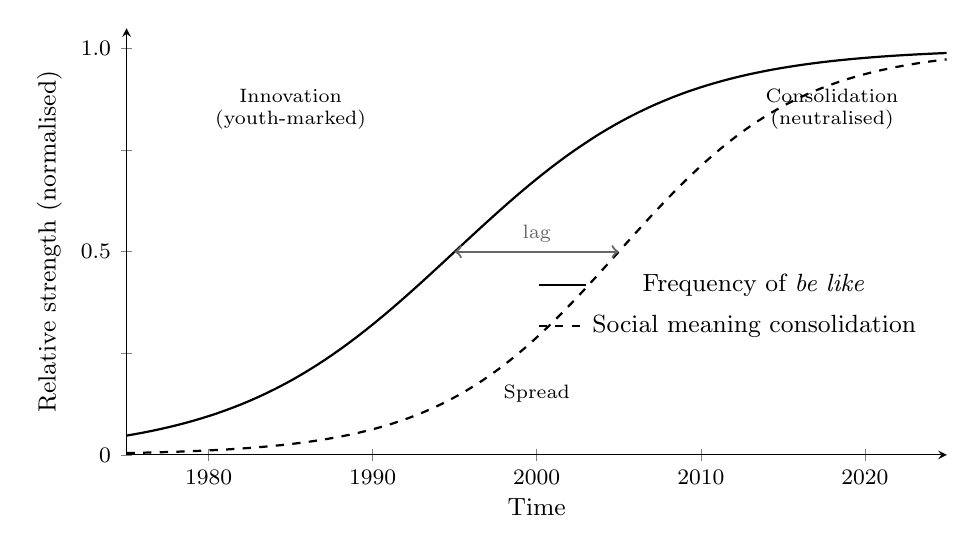
\begin{tikzpicture}
\begin{axis}[
    width=12cm,
    height=7cm,
    xlabel={Time},
    ylabel={Relative strength (normalised)},
    xmin=1975, xmax=2025,
    ymin=0, ymax=1.05,
    xtick={1980, 1990, 2000, 2010, 2020},
    x tick label style={/pgf/number format/1000 sep={}},
    ytick={0, 0.25, 0.5, 0.75, 1.0},
    yticklabels={0, , 0.5, , 1.0},
    axis lines=left,
    xlabel style={at={(0.5,-0.08)}, font=\small},
    ylabel style={font=\small},
    tick label style={font=\footnotesize},
    legend style={
        at={(0.98,0.35)},
        anchor=east,
        font=\small,
        draw=none,
        fill=none,
        row sep=3pt
    },
    clip=false
]

% Frequency curve (S-curve, earlier)
% Logistic: 1 / (1 + exp(-k(x - x0)))
\addplot[
    thick,
    black,
    domain=1975:2025,
    samples=100
] {1 / (1 + exp(-0.15*(x - 1995)))};
\addlegendentry{Frequency of \textit{be like}}

% Social meaning consolidation curve (S-curve, lagged)
\addplot[
    thick,
    black,
    dashed,
    domain=1975:2025,
    samples=100
] {1 / (1 + exp(-0.18*(x - 2005)))};
\addlegendentry{Social meaning consolidation}

% Lag annotation
\draw[<->, thick, black!60] (1995, 0.5) -- (2005, 0.5);
\node[font=\scriptsize, above, black!60] at (2000, 0.5) {lag};

% Phase labels
\node[font=\scriptsize, align=center] at (1985, 0.85) {Innovation\\(youth-marked)};
\node[font=\scriptsize, align=center] at (2000, 0.15) {Spread};
\node[font=\scriptsize, align=center] at (2018, 0.85) {Consolidation\\(neutralised)};

\end{axis}
\end{tikzpicture}
\caption{Schematic relationship between frequency rise and social-meaning consolidation for quotative \textit{be like}. Both curves represent relative trajectories rather than measured values; the frequency curve abstracts over attested data patterns, the consolidation curve reflects the qualitative pattern. The lag between curves reflects the expected period during which the form carries strong indexical value (youth, informality); consolidation marks the attenuation of marked social meaning as the form becomes the community default.}
\label{fig:diffusion-meaning}
\end{figure}

The quotatives case is a site where predictive processing and social indexing co-align, each reinforcing the other. The discourse routines of informal narrative make quotative contexts highly predictable~-- you know a quotative is coming before it arrives. That predictability encourages rapid uptake; rapid uptake feeds entrenchment; entrenchment makes the form even more predictable next time. Meanwhile, social indexing adds a parallel reinforcement loop: forms that mark in-group identity get used more in the high-frequency contexts where identity matters, which strengthens both the processing advantage and the social signal. The braid tightens because the strands pull in the same direction.

Online processing pressures~-- prediction, retrieval ease, reduced production cost under repetition~-- preferentially reinforce some cluster features over others. The features that are easy to predict, easy to produce, and easy to retrieve are the ones that survive and spread. That selective reinforcement keeps the category coherent across time and speakers. Processing isn't just something that happens to categories; it's one of the mechanisms that maintains them.



\subsection{What if a mechanism were absent?}

A stress test: what if we removed each stabiliser in turn? If the braid is genuinely explanatory, no single strand should suffice.

If processing economy were the only stabiliser, we'd expect the shortest form to win regardless of discourse function. But \mention{say} is shorter than \mention{be like}, and it doesn't dominate.

If expressive fit were the only stabiliser, we'd expect any form that introduces vivid quotation to spread equally. But quotatives with pejorative associations, or unfashionable indexical value, don't spread even when they fit the discourse need.

If social indexing were the only stabiliser, we'd expect pure fashion effects: quotatives rising and falling with generational taste, cycling over a decade or two. But \mention{be like} has been stable for four decades, long past a typical lexical-fashion cycle.

If transmission were the only stabiliser, we'd expect all forms heard in childhood to survive. But archaic quotatives like \mention{quoth} or reduced variants that never gained social cachet don't persist.

If acquisition and cohort effects were the only stabiliser, we'd expect forms entrenched early to persist within individuals but fail to generalise across the community. Yet quotatives that never achieve narrative or indexical value don't survive beyond the cohorts that first encountered them.

The observed pattern~-- cross-linguistic convergence on light, expressive, youth-indexed, narratively deployed quotatives~-- requires the full braid. If one strand did all the work, this chapter would be an email. No single mechanism is sufficient.

These counterfactuals generate testable predictions. Table~\ref{tab:perturbation-grid} summarises the expected empirical signatures if each stabiliser were selectively attenuated while others remained intact.

\begin{table}[htbp]
\centering
\scriptsize
\begin{tabular}{@{}p{2.5cm}ccccc@{}}
\toprule
\makecell[l]{\textbf{Mechanism}\\\textbf{attenuated}} & \makecell{\textbf{Freq.}} & \makecell{\textbf{Judgment}\\\textbf{variance}} & \makecell{\textbf{Social}\\\textbf{meaning}} & \makecell{\textbf{Cross-context}\\\textbf{transfer}} & \makecell{\textbf{Historical}\\\textbf{trajectory}} \\
\midrule
Processing economy $\downarrow$ & gradual $\downarrow$ & slight $\uparrow$ & retained & reduced & slowed spread \\
\addlinespace
Expressive fit $\downarrow$ & stable $\rightarrow$ gradual $\downarrow$ & moderate $\uparrow$ & weakened & reduced & stalled expansion \\
\addlinespace
Social indexing lost & stable & stable & neutralised & stable & age-grading only \\
\addlinespace
Acquisition disrupted & cohort $\downarrow$ & high $\uparrow$ & fragmented & patchy & generational gaps \\
\addlinespace
Transmission blocked & rapid $\downarrow$ & low within cohort & fossilised & retained & arrested \\
\bottomrule
\end{tabular}
\caption{Predicted empirical signatures of mechanism attenuation. Each row specifies observable consequences if a single stabiliser were weakened while others remained intact.}
\label{tab:perturbation-grid}
\end{table}


\subsection{Cross-linguistic convergence}

Similarity across languages can arise by two routes: diffusion of a particular form across related varieties, or convergent development under shared stabilising pressures. Both are relevant here.

Japanese, Turkish, German, and English share almost nothing: different word orders, different morphological profiles, different sociolinguistic ecologies. Yet they converge on similar quotative innovations. Within English varieties, the global spread of \mention{be like} suggests diffusion with local adaptation. Across unrelated languages, innovative quotatives arise from different lexical sources but converge on a similar functional territory. The maintenance view predicts this dual pattern: a form may travel, but even when it doesn't, similar stabilisers recruit new material into the same niche.

The temporal pattern is striking. In English, \mention{be like} was first attested in the US in 1982 \autocite{butters1982}, at least seven years before it appeared in any other variety \autocite{buchstaller2014}. It reached the UK by 1994 \autocite{andersen1996}, New Zealand and Canada by 1995 \autocite{baird2001,tagliamonteH1999}, Australia by 1997 \autocite{winter2002}. The form then appeared in outer-circle Englishes: Singapore, Hong Kong, Kenya, Jamaica, the Philippines. By the 2000s, it had global attestation across typologically diverse contact varieties.

One obvious hypothesis is media transmission. The `Valley Girl' stereotype, propelled into popular culture by Frank Zappa's 1982 song and subsequent Hollywood films, made \mention{be like} audible to millions. But \textcite{buchstaller2014} finds little evidence for straightforward media-driven borrowing. Speakers rarely associate \mention{be like} with media stereotypes; the form's linguistic conditioning varies across localities in ways inconsistent with uniform transmission; and the development pattern shows `transformation under transfer'~-- local adaptation of a form that arrived from elsewhere~-- rather than passive copying.

The stronger hypothesis is convergent development under similar functional pressures. The semantic-pragmatic sources for innovative quotatives~-- deictic markers, movement verbs, approximation expressions~-- recur across typologically unrelated languages \autocite{guldemann2008}. German recruits \mention{so} (a deictic), Japanese recruits \mention{tte} (a reduced quotative verb), Turkish recruits \mention{diye} (a converb), English recruits \mention{like} (an approximator). The sources differ, but the functional territory is the same: introducing vivid, non-verbatim re-enactment in informal narrative.

The convergence is not lexical; it's structural. The stabilising mechanisms are the same:

\begin{itemize}
   \item Processing economy favours light forms.
   \item Expressive fit favours vague-reference quotatives.
   \item Social indexing favours youth-marked forms.
   \item Transmission dynamics favour high-frequency, contextually salient forms.
\end{itemize}

Wherever these mechanisms operate~-- and they operate everywhere humans tell stories to each other~-- the same type of quotative emerges. The category is not defined by a shared etymon or a universal grammar rule. It's stabilised by a convergent mechanism profile.

A caution about what convergence shows. Similar surface profiles suggest convergent \emph{problems}~-- similar functional pressures, similar communicative needs. They don't automatically demonstrate the same underlying stabilisers at the same relative weights. In one ecology, processing economy may dominate; in another, social indexing may do more work. German \mention{so} remains more register-restricted than English \mention{be like}, even though both serve the same niche~-- which suggests that the social-indexing pressures differ, even as the processing pressures align. Convergent profiles are evidence that the \emph{type} of mechanism is similar; the specific braid may still vary across ecologies.

This is what \enquote{same category across languages} means in the maintenance view: convergent stabilisation, the clustering that emerges when similar mechanisms operate under similar pressures. The convergence is predictable: if processing economy and expressive fit are universal~-- all humans favour light forms under production pressure, all humans need vague-reference quotatives for storytelling~-- then similar sociolinguistic dynamics will produce similar outcomes wherever they operate. But \enquote{similar outcomes} needn't mean identical mechanisms. The framework predicts family resemblance in the stabilising story, not clones.


\subsection{How deep do mechanisms go?}

The stress test confirms necessity: no single strand suffices. A deeper question: what \emph{are} these mechanisms? The stabilisers just described~-- processing economy, expressive fit, social indexing, transmission dynamics~-- might look like endpoint explanations. But mechanisms have mechanisms. Each stabiliser can be decomposed causally (what underlies it?) and mereologically (what are its parts?). The decomposition reveals the multi-level architecture of category maintenance.

\subsubsection{Causal depth}

Take the robust finding that young women lead quotative innovation \autocite{labov2001,tagliamontedarcy2004}. This isn't a brute fact. It plausibly traces back to social-psychological and network structure.

Young women's peer networks are often reported to be denser and more multiplex than young men's, especially in adolescence \autocite{milroy1987}. Dense networks mean more linguistic input, more accommodation pressure, faster entrenchment of shared forms. Multiplex ties~-- relationships serving multiple social functions~-- mean higher interactional stakes and stronger motivation to coordinate. When your interlocutor is also your classmate, neighbour, and confidante, alignment is more consequential than with a stranger.

But why dense networks in adolescence at all? Developmental psychology provides the next level down. Adolescence is the period of separation-individuation, when peer orientation overtakes parent orientation \autocite{erikson1968}. The social structure of schooling concentrates age-cohorts in prolonged daily contact~-- co-location plus time produces the network density that shapes linguistic input. Identity construction becomes primary: you need to differentiate from your parents while affiliating with your peers. Linguistic innovation serves both goals simultaneously~-- it marks in-group solidarity and out-group distinction.

Why these developmental facts? At this level we're sketching distal shaping of the selection environment rather than a direct mechanistic chain: evolutionary pressures on coalition formation, cultural transmission of gender norms, economic structures that extend education and delay labour-market entry. These factors may shape network structure, which shapes input frequency, which shapes entrenchment. \enquote{Young women lead quotative change} isn't a stipulation; it's the surface manifestation of a causal cascade~-- though how far down the cascade runs remains an open empirical question.

A caution: this is a \emph{possible} depth path, not a confirmed one. The evidence requirements tighten as we descend levels. The sociolinguistic pattern (young women leading) is robust; the network-density explanation is well-supported; the developmental-psychology account is plausible but less directly tested; the evolutionary and economic claims are speculative. The framework permits depth without requiring it~-- what matters is that the mechanism at each level be genuinely explanatory, not that every level be equally confirmed. Readers who find the deeper levels overreaching can stop at network density without losing the main argument; that level already provides a complete stabiliser story for the quotative case.

How far down should linguistic explanation go? Far enough to explain the clustering at the level we care about. For the quotative case, the clustering is grammatical: first-person preference, youth association, non-verbatim content. The mechanisms are social and cognitive: network density, identity work, processing pressure, entrenchment dynamics. We \emph{could} trace further~-- to neuroscience, to evolutionary biology~-- but the grammatical clustering is already explained. The framework is level-agnostic: it says look for mechanisms that produce clustering, without dictating which level to bottom out at.

\subsubsection{Mereological structure}

The same decomposition applies to parts, not just causes. \enquote{Transmission} sounds like a single mechanism, but it's a composite.

Production processes come first: lexical selection (choosing \mention{be like} over \mention{say}), which involves activating competitors, weighting by frequency, and filtering by context~-- register, addressee, narrative function. Then syntactic planning: slotting the copula and predicative into a quotative frame. Then phonetic realisation: the actual articulation of \mention{like}.

The signal bridges production and perception: acoustic properties, prosodic packaging (the characteristic intonation contour that marks enactment).

Perception processes follow: segmenting the stream, recognising words, parsing the construction, assigning category membership. Each is a sub-mechanism with its own structure~-- word recognition draws on frequency-weighted access, construction parsing draws on facilitated patterns, category assignment draws on distributional learning.

Each encounter updates the conditions for future production: encoding this token in context (acoustic trace, syntactic frame, pragmatic function, social co-occurrence~-- who said it, to whom, with what stance), facilitating future reconstruction of similar forms, strengthening form-function associations. The listener becomes a speaker whose lexical selection is now shifted slightly toward the form just heard.

Social processes interleave throughout: accommodation (matching the interlocutor), identity projection (signaling youth and informality), stance-taking (performing enactment rather than merely reporting). \textcite{pickering2004} model alignment as automatic priming; \textcite{Eckert2012} situates it in identity construction. Both are part of what \enquote{transmission} means.

The mereological lesson: even the mechanisms introduced in Chapter~\ref{ch:kinds-without-essences}~-- acquisition, entrenchment, alignment, functional pressure~-- are not atoms. They're composites with internal structure. When we say \enquote{transmission maintains the category}, we're compressing a multi-part process into a single term. The term is still explanatory~-- it picks out a real causal structure~-- but the structure is articulated, not monolithic. The point here is the compositionality of transmission, not adjudication between competing models of priming versus identity-driven alignment.

\subsubsection{What this means for explanation}

The depth and structure of mechanisms matter for two reasons.

First, they reveal where intervention is possible. If transmission depends on particular memory processes, then anything that disrupts those processes~-- reduced input frequency, competing forms, register restriction~-- will weaken the mechanism. Knowing the parts tells you where the leverage points are. This is why Chapter~\ref{ch:failure-modes} on failure modes will matter: category dissolution happens when sub-mechanisms fail, and understanding which sub-mechanisms are failing requires knowing what they are.

Second, they connect linguistic explanation to the broader sciences. The causal depth that runs from \enquote{young women lead change} through network density to developmental psychology to evolutionary pressures is where linguistics fits into the larger picture. The maintenance view doesn't require every linguist to become a psychologist or evolutionary biologist. But it does make explicit that grammatical categories are maintained by mechanisms that ultimately ground in facts about human cognition, social structure, and history. The framework is continuous with the rest of science, not sealed off from it.

\subsubsection{Mechanisms as categories, categories as mechanisms}

A deeper point emerges from this decomposition.

If categories are projectible clusters stabilised by mechanisms, and if the mechanisms themselves are projectible clusters stabilised by further mechanisms, then mechanisms are categories. \term{Processing economy} is a category~-- it bundles properties (reduced forms, high frequency, resistance to analogical pressure) that cluster reliably because of underlying neural and memory constraints. \term{Social indexing} is a category~-- it bundles properties (youth association, in-group marking, register restriction) maintained by identity construction and network dynamics. The mechanisms we invoke to explain quotative stability are themselves HPC kinds, maintained by their own braids of stabilisers.

The stabilisation, moreover, is reciprocal.

Quotatives don't just \emph{use} processing economy~-- they \emph{maintain} it. Every time a speaker produces \mention{be like}, that token is input to the conditions that ground processing economy. The form's high frequency reinforces the facilitation that makes high-frequency forms easier to produce~-- not by rewriting the rules of activation, but by keeping the relevant usage ecology dense. The mechanism depends on the category for its continued operation just as the category depends on the mechanism, which, like a sourdough starter, goes mouldy if neglected.

Social indexing exhibits the same reciprocity. It isn't just something that quotatives \emph{do}; it is partly \emph{built out of} the patterned circulation of particular quotative variants. The indexical field that makes youth-associated forms socially meaningful persists because forms like \mention{be like} repeatedly occur with those personae and stances. The indexical field is an emergent structure sustained by the form's patterned social distribution. You get \enquote{youth style} the way you get a trail in the woods: by people walking it. Remove a major, high-salience contributor to that pattern and the local indexical alignment would likely attenuate. In that sense, the category and the mechanism co-construct each other.

This is not a vicious circle; it's a self-organising dynamic~-- precisely the homeostatic structure that gives HPC kinds their stability. Categories shape what gets entrenched, and entrenchment shapes which categories survive, so each stabilises the other. Figure~\ref{fig:causal-loop} visualises this reciprocal structure.

\begin{figure}[htbp]
\centering
\begin{tikzpicture}[
    mechanism/.style={rectangle, draw, thick, minimum width=2.8cm, minimum height=1.2cm, align=center, font=\small},
    category/.style={ellipse, draw, thick, minimum width=3.2cm, minimum height=1.6cm, align=center, font=\small\bfseries},
    arrow/.style={-{Stealth[length=2.5mm]}, thick},
    looparrow/.style={-{Stealth[length=2.5mm]}, thick, color=blue!70!black},
    plus/.style={font=\scriptsize\color{blue!70!black}},
    looplabel/.style={font=\tiny, color=blue!70!black}
]

% Central node
\node[category] (cat) {QUOTATIVE\\CATEGORY};

% Mechanism nodes
\node[mechanism, above left=1.8cm and 2.2cm of cat] (proc) {Processing\\economy};
\node[mechanism, above right=1.8cm and 2.2cm of cat] (soc) {Social\\indexing};
\node[mechanism, below left=1.8cm and 2.2cm of cat] (acq) {Acquisition \&\\entrenchment};
\node[mechanism, below right=1.8cm and 2.2cm of cat] (trans) {Transmission\\dynamics};

% Bidirectional arrows: mechanisms <-> category
% Processing economy
\draw[arrow] (proc.south east) -- node[plus, above, pos=0.4] {+} (cat.north west);
\draw[arrow] (cat.north west) ++ (0.15, 0.1) -- node[plus, below, pos=0.6] {+} ([xshift=0.3cm]proc.south east);

% Social indexing
\draw[arrow] (soc.south west) -- node[plus, above, pos=0.4] {+} (cat.north east);
\draw[arrow] (cat.north east) ++ (-0.15, 0.1) -- node[plus, below, pos=0.6] {+} ([xshift=-0.3cm]soc.south west);

% Acquisition
\draw[arrow] (acq.north east) -- node[plus, below, pos=0.4] {+} (cat.south west);
\draw[arrow] (cat.south west) ++ (0.15, -0.1) -- node[plus, above, pos=0.6] {+} ([xshift=0.3cm]acq.north east);

% Transmission
\draw[arrow] (trans.north west) -- node[plus, below, pos=0.4] {+} (cat.south east);
\draw[arrow] (cat.south east) ++ (-0.15, -0.1) -- node[plus, above, pos=0.6] {+} ([xshift=-0.3cm]trans.north west);

% Inter-mechanism arrows
\draw[looparrow] (proc.south) to[bend right=20] node[plus, left, pos=0.5] {+} (acq.north);
\draw[looparrow] (soc.south) to[bend left=20] node[plus, right, pos=0.5] {+} (trans.north);

% Reinforcing loop indicators
\node[looplabel] at ([xshift=-1.1cm, yshift=0.3cm]cat.north) {\footnotesize$\circlearrowright$\tiny R};
\node[looplabel] at ([xshift=1.1cm, yshift=0.3cm]cat.north) {\footnotesize$\circlearrowright$\tiny R};
\node[looplabel] at ([xshift=-1.1cm, yshift=-0.3cm]cat.south) {\footnotesize$\circlearrowright$\tiny R};
\node[looplabel] at ([xshift=1.1cm, yshift=-0.3cm]cat.south) {\footnotesize$\circlearrowright$\tiny R};

% External inputs
\node[font=\small, below=3.8cm of cat] {External inputs: memory architecture, network structure, developmental ecology};

\end{tikzpicture}
\caption{Reciprocal maintenance of a grammatical category. Each mechanism both stabilises and is sustained by the category it maintains. Arrows marked + indicate reinforcing relationships; $\circlearrowright$R marks reinforcing feedback loops.}
\label{fig:causal-loop}
\end{figure}

A contrast case sharpens the point. Consider the traditional category \term{particle}~-- a wastebasket label for uninflected words that don't fit elsewhere: \mention{up} in \mention{look up}, \mention{to} in infinitives, \mention{not}, sentence-final \mention{eh}. Does this cluster survive a maintenance audit? The properties don't co-occur reliably: \mention{up} takes complements; infinitival \mention{to} doesn't; \mention{not} has scope properties shared by neither. There's no common acquisition pathway: children learn verb-particle constructions, infinitives, and negation at different times, through different input distributions. There's no processing signature: reaction-time studies don't show \enquote{particle} effects that generalise across subtypes. There's no transmission dynamic: speakers don't acquire \enquote{particle-hood} as a generalisable category; they acquire constructions that happen to contain uninflected words. Predictions trained on one subtype (verb-particles) fail to transfer to another (infinitival \mention{to}). The label exists; the mechanism-maintained kind doesn't. Failure of reciprocal maintenance looks exactly like this: the supposed category doesn't exercise a shared mechanism, and no shared mechanism makes the category projectible. Chapter~\ref{ch:failure-modes} develops such failure modes systematically; here, the contrast case shows that the quotative analysis isn't analogy-by-enthusiasm~-- it identifies genuine stabilisation that \term{particle} lacks.

The quotative category is also a mechanism in the larger kinds that contain it. Quotatives are part of what maintains \term{narrative discourse structure}~-- they enable the vivid re-enactment that makes storytelling work. They are part of what maintains \term{youth register}~-- the forms that index adolescent identity and solidarity. They are part of what maintains \term{informal speech} as a recognisable variety~-- the cluster of features that signals casualness, immediacy, peer context. And again, the stabilisation is reciprocal: narrative structure provides the discourse ecology in which quotatives function; youth register provides the social meaning that quotatives carry; informal speech provides the register niche that quotatives occupy.

So the hierarchy runs both ways. Downward: quotatives are maintained by mechanisms (processing, acquisition, social indexing, transmission), which are themselves maintained by deeper mechanisms (memory architecture, developmental psychology, network structure). Upward: quotatives are mechanisms in larger categories (narrative structure, youth register, informal speech), which are themselves mechanisms in still larger kinds (discourse genres, sociolinguistic repertoires, speech communities). And at every level, the stabilisation is bidirectional: each element both depends on and sustains the elements above and below it.

The distinction between \enquote{category} and \enquote{mechanism} is perspectival, not ontological. What counts as a category at one scale is a mechanism at another. What stabilises quotatives is stabilised by quotatives.

A sceptic might ask: if every mechanism is itself a category maintained by further mechanisms, what grounds the explanatory chain? Two responses are available.

The interventionist answer: we stop when we reach mechanisms whose disruption would change the clustering in predictable ways. This is already implicit in the robustness tests above (\enquote{What if a mechanism were absent?}). A mechanism earns its keep by specifying where intervention would bite. If we can say \enquote{reduce input frequency and the category weakens}, we have a mechanism. The grounding is not metaphysical bedrock; it's causal tractability.

The anti-foundationalist answer: explanatory chains don't need bedrock. The regress objection assumes that justification must terminate in self-evident foundations~-- but coherentist epistemologies reject this. What matters is that the explanatory network is mutually supporting and empirically fruitful. Each mechanism explains the categories above it and is explained by the mechanisms below it; the network as a whole is tested by whether it generates accurate predictions. The demand for a single ultimate ground is a vestige of foundationalist philosophy that the sciences have largely abandoned.

Both responses are compatible. The framework is interventionist in practice and anti-foundationalist in principle. For any given explanatory purpose, we stop where the causal leverage is~-- but we don't pretend that stopping point is metaphysically privileged.


\section{A second case: filler-gap and independent relative \mention{whose}}
\label{sec:7:filler-gap-whose}

The quotative case shows mechanisms maintaining a category primarily from above~-- from the functional and social pressures that keep the clustering clustered. But a sceptic might wonder: is this just sociolinguistics dressed in HPC clothing? A second case answers that challenge by showing mechanisms maintaining a construction from below~-- from incremental parsing, recoverability constraints, and genre ecology rather than from social indexing or cohort transmission.

The evidential asymmetry matters: the quotative case rests on decades of variationist data; the \mention{whose} case that follows rests on attestation data. The framework predicts high inter-speaker variation and sensitivity to discourse context, but this remains to be tested. For now, the \mention{whose} case should be read as a \emph{prediction} of the framework rather than a confirmation on par with quotatives.

\subsection{The filler-gap mechanism}

When you hear \mention{Which book did Mary say that John read \_\_?}, you track a displaced constituent: \mention{which book} is the filler, and the gap after \mention{read} is where it's interpreted. This filler-gap dependency spans clause boundaries, requires memory, and operates across surface variation~-- open interrogatives, relative clauses, clefts.

As mentioned in Chapter~\ref{ch:projectibility}, \citet{boguraev2025} used causal interventions to test whether language models learn a shared mechanism across these construction types. They do: a mechanism learned on embedded open interrogatives transfers to produce filler-gap behaviour in clefts. The result is a proof of concept~-- showing how mechanistic generalisation could work in principle~-- rather than direct evidence about human parsing (see also \citealt{pistotti2025gaps} on robust filler-gap generalisation in parasitic gap environments). But the structural dependency projects even when the surface constructions differ, which is what mechanistic kindhood predicts.

\subsection{Independent relative \mention{whose}: a gap that isn't}

A case study deepens the point. \citet{hankamer1973whose} claimed that English lacks independent relative \mention{whose}~-- forms like \mention{a woman whose was straight} where the possessum is elided. Their constructed examples are indeed ungrammatical: \mention{*The guy whose you saw banging at the window...} fails. For fifty years, the construction was treated as a paradigm gap~-- a systematic lacuna in the grammar.

But the gap may be illusory. \citet{reynolds2024whose} documents attestations spanning seven centuries, from Middle English manuscripts to contemporary academic prose: \mention{a friend of whose had told us of the accident}; \mention{those whose are not}. The construction is vanishingly rare~-- on the order of once per hundred million words in large corpora~-- but attested in edited sources, particularly academic and journalistic prose.\footnote{The grammaticality judgments remain disputed. \textcite{reynolds2024whose} is a preprint, and native-speaker intuitions vary. The epistemic status is accordingly tentative: suggestive evidence that the mechanism is there, not conclusive proof.} The point isn't that the earlier judgment was irrational; the point is that a mechanism-first view predicts that apparent gaps can be ecological artefacts of licensing contexts.

What maintains this construction despite its extreme rarity? The same mechanisms that maintain other filler-gap constructions~-- but operating under unusually stringent conditions.

\subsection{Filler-gap stabilisers}

\textbf{Filler-gap processing.} Independent relative \mention{whose} is a filler-gap construction. \mention{Whose} fills a gap in subject or complement position: \mention{a woman whose \_\_ was straight}. The displaced constituent must be tracked across clause structure and resolved at the gap site. This is the same cognitive operation that underlies relative clauses, open interrogatives, and clefts~-- the mechanism that Boguraev et al. showed transfers across construction types. Here, as with quotatives, mechanisms at different scales~-- cognitive, interactional, institutional~-- interact to maintain the construction.

The filler-gap mechanism is maintained by processing pressures. Incremental parsing requires tracking dependencies as they unfold; memory constraints favour local resolution; prediction mechanisms anticipate gap sites. These pressures apply every time a speaker processes a relative clause or an interrogative. The mechanism is exercised constantly, even if independent \mention{whose} is exercised rarely.

\textbf{Information structure.} But filler-gap processing alone isn't sufficient. Independent \mention{whose} faces an additional burden: the elided possessum must be recoverable. This is what \citet{reynolds2024whose} calls the \enquote{double anaphora} requirement~-- the hearer must simultaneously recover the possessor (from the relative clause antecedent) and the possessum (from discourse context).

Three information-structural configurations license this recovery. Under \emph{contrastive parallelism}, the possessum is established in a preceding clause and the \mention{whose} clause contrasts with it: \mention{I knew someone whose greatest love affair was with objects, another whose was with books, and a third whose was with ideas.} Under \emph{deictic anchoring}, a demonstrative directly points to the possessum: \mention{The man whose these are hath gotten me with child.} Under \emph{structural integration}, the possessum appears as head of the phrase containing \mention{whose}: \mention{a friend of whose had told us of the accident.}

These aren't arbitrary conditions. They're the configurations that satisfy the recoverability constraint~-- the same constraint that governs ellipsis generally. The information-structural mechanism is independent of the filler-gap mechanism, but both must be satisfied for the construction to succeed~-- only when both mechanisms clear their thresholds does the construction clear the grammaticality threshold.

\textbf{Discourse ecology.} Why did identity-of-sense stranding (where the elided possessum shares only sense with an antecedent) emerge only in the 1990s, when identity-of-reference stranding (where it shares reference) has existed since Middle English? Plausibly not because the grammar changed, but because the discourse ecology changed.

Academic and journalistic prose favours list-like enumerations and explicit contrast sets: \mention{patients whose symptoms improved versus those whose didn't}. These registers build the contrastive parallelism that licenses possessum recovery. The construction plausibly became more available when the discourse patterns that license it became conventionalised in particular genres. The mechanism was always there; the licensing environment wasn't.

A brief stress test: if filler-gap processing were absent, independent \mention{whose} would be impossible~-- but so would all relative clauses, interrogatives, and clefts. If information-structural licensing were absent, the construction would fail even in contrastive contexts. The construction's rarity isn't mechanism weakness; it's licensing scarcity. Both cognitive mechanism and pragmatic licensing are necessary; neither alone suffices.

I treat independent relative \mention{whose} as one English instantiation of a broader independent possessive-relative profile, so cross-linguistic parallels are predictions about the mechanism package rather than claims of identical surface syntax.

\textbf{Cross-linguistic convergence.} German and Japanese~-- despite radically different syntactic structures~-- appear to show similar information-structural constraints on independent possessive relatives:

\begin{quote}
\textbf{German:} \mention{Meins funktionierte, aber ich kenne jemanden, dessen nicht funktionierte.} (`Mine was working, but I know someone whose wasn't.')~-- licensed by contrastive parallelism.\\
\textbf{German:} *\mention{Die Person, dessen du vergessen hast, ist mein Cousin.} (`The person whose you forgot is my cousin.')~-- fails without parallelism.\\
\textbf{Japanese:} \mention{Watashi-no-wa ugoite-ita ga, ugoite-ina-katta hito-mo shitte-iru.} (`Mine was working, but I also know someone whose wasn't.')~-- licensed by contrastive parallelism.\footnote{The Japanese example is the author's judgment, confirmed with native-speaker consultants. Systematic corpus study of Japanese possessive stranding remains to be done.}
\end{quote}

The pattern may mirror English, though systematic study is needed: stranding succeeds under contrastive parallelism and fails without it. If the parallel holds, the constraints are not language-specific accidents but consequences of how filler-gap processing interacts with discourse accessibility.

The surface structures differ~-- German has rich case marking, Japanese is head-final, English has relatively impoverished case and is head-initial~-- but the underlying mechanisms (incremental parsing, memory constraints, communicative pressure for recoverability) are constants, and the constraints on independent possessive relatives track those constants, not the surface variation.

The \mention{whose} case illustrates the chapter's central argument: a shared cognitive mechanism (filler-gap processing) operates under a specific constraint profile (information-structural licensing), and that profile recurs across typologically unrelated languages because the constraints track universal processing pressures, not language-specific syntax. The maintenance is reciprocal: filler-gap constructions exercise the processing mechanism that makes them possible, while the mechanism makes the constructions processable in turn. \enquote{Labels aren't mechanisms} means exactly this in practice: the label \enquote{ungrammatical} predicted nothing; the mechanism story predicts exactly when the construction succeeds and when it fails.

We should also expect the constraints to pattern with experience, because the construction depends on licensing conditions that are themselves unevenly distributed. Speakers with greater exposure to the contrastive-parallelism registers~-- academic prose, formal journalism~-- may find independent \mention{whose} more accessible than speakers without such exposure. Differential mastery is not a defect of the grammar; it's a prediction of the maintenance view.

The filler-gap case shows the same reciprocal structure as quotatives. Every relative clause, every interrogative, every cleft is input to the conditions that sustain filler-gap processing. The mechanism is real because it's kept alive by the constructions it serves.


\section{How to test whether a mechanism is real}
\label{sec:7:robustness-tests}

The biological approach gives us a natural framework for testing mechanistic claims. Not hand-waving that \enquote{entrenchment maintains the category}, but operational tests that distinguish genuine causal structure from convenient labels. The tests are ordered here by inferential strength~-- from interventions that most directly force reality-commitments to distributional patterns that support but don't compel them.

\textbf{1. Intervention and ablation.} The strongest evidence for a mechanism is that disrupting it changes the outcome. In linguistics, this means: disrupting input patterns (acquisition perturbation), shifting register ecology (contact situations, code-switching), or computationally lesioning a processing component (as Boguraev et al.\ did for filler-gap dependencies). If the category reshapes in predictable ways when the hypothesised stabiliser is weakened, the mechanism is real. \emph{What could mislead us:} interventions may have unintended side effects; apparent reshaping may reflect compensation by other mechanisms rather than loss of the target stabiliser. Chapter~\ref{ch:failure-modes} addresses how to distinguish genuine mechanism loss from compensatory masking.

\textbf{2. Cross-construction transfer.} If a mechanism is real, competence in one construction should predict performance in another that shares the mechanism. The Polish aspect models show this: training on one verb subset, testing on another, predictions transfer. Boguraev et al.\ showed it for filler-gap: a mechanism learned on interrogatives transfers to clefts. Transfer is evidence that category boundaries track causal structure, not just filing conventions. \emph{What could mislead us:} transfer may reflect surface similarity rather than shared mechanism; conversely, lack of transfer may reflect task demands rather than mechanism absence.

\textbf{3. Predictive constraints under licensing conditions.} If a construction depends on specific licensing conditions, success should spike when those conditions are met and fail when they're not. The \mention{whose} case exemplifies this: stranding succeeds under contrastive parallelism and fails without it. If we can predict exactly when the construction will be licensed, the mechanism story is doing real work. \emph{What could mislead us:} licensing conditions may be more complex than hypothesised; apparent success may reflect memorised exemplars rather than productive use of the mechanism.

\textbf{4. Ecological rarity.} Rarity is not disconfirming if the licensing ecology is rare. \mention{Whose}-stranding appears once per hundred million words~-- but the information-structural configurations that license it are themselves rare in most corpora. Rarity becomes disconfirming only when predicted licensing contexts are common yet the construction still doesn't appear. This test requires distinguishing \emph{mechanism absence} from \emph{licensing scarcity}~-- a distinction the \mention{whose} case makes vivid. \emph{What could mislead us:} corpus sampling may miss the relevant registers; rarity may reflect stigmatisation rather than mechanism weakness.

\textbf{5. Reciprocal maintenance signatures.} If mechanisms and categories co-construct each other, we should observe bidirectional effects: categories shaping what gets entrenched, entrenchment shaping what categories survive. Panel data on quotatives show this: apparent-time change in one direction (younger speakers use \mention{be like} more) co-occurs with cohort effects in the other (speakers carry their adolescent inventory into adulthood). The signature is mutual shaping, not unidirectional causation. \emph{What could mislead us:} correlation may mimic reciprocity; what looks like bidirectional causation may be two effects of a common cause.

\textbf{6. Distributional and attestation coherence.} The weakest test, but still probative: if a category is maintained by stable mechanisms, the distributional cues for category membership should be mutually predictive across registers, time periods, and populations. Cue bundles that fragment under replication are evidence against mechanism; cue bundles that remain coherent are evidence for it. \emph{What could mislead us:} distributional coherence may reflect historical accident rather than ongoing maintenance; attestation may be artefact of corpus composition.

No single test is decisive. Mechanism claims earn credibility when two or more tests converge~-- when intervention effects, transfer patterns, and licensing predictions all point to the same underlying causal structure. Single-test reasoning invites overclaim; triangulation constrains it.

In practice, these tests translate into specific research designs: psycholinguistic tasks (reaction time, eye-tracking, ERPs) for processing facilitation; register-ecology sampling for distributional coherence; controlled acceptability work designed to manipulate licensing contexts; corpus perturbation and counterfactual modelling for historical change; computational causal interventions for mechanism isolation. The tests are not philosophical abstractions; they are guides to experimental and corpus-analytic practice.

A practical recipe, in prose: (1) Identify the cluster~-- what properties co-occur? (2) Propose stabilisers at two or three levels~-- cognitive, social, transmissional. (3) Derive at least one intervention or natural-experiment prediction~-- if we weaken this stabiliser, how should the clustering change? (4) Check whether the predicted reshaping is observed~-- in acquisition data, contact situations, or experimental manipulations. (5) Triangulate~-- does independent evidence from transfer, licensing, or distribution converge on the same mechanism? If the predictions hold across tests, the stabiliser is load-bearing. If they fail, revise or discard.

These tests certify mechanisms when they work. Chapter~\ref{ch:failure-modes} shows how to diagnose when the tests themselves mislead~-- when false positives, compensation effects, and ecological confounds create the appearance of mechanism where none exists, or mask genuine mechanisms that the tests fail to detect.


\section{Degrees of projectibility}
\label{sec:7:degrees-projectibility}

The stabilising story explains why projectibility comes in degrees.

A category deep in a single basin~-- that is, supported by multiple aligned stabilisers (entrenchment, transmission, functional pressure, social reinforcement), all pulling in the same direction~-- is strongly projectible. You can learn about nouns from a few exemplars and generalise reliably to new nouns. The mechanisms reinforce each other across timescales.

A category in an overlap region~-- where mechanisms pull in different directions, or where entrenchment is weak~-- is weakly projectible. Predictions work for typical cases but fail for edge cases. The degree of projectibility tracks the degree of mechanistic support.

A label with no mechanisms behind it is not projectible at all. A wastebasket category defined by what it's not should fragment under the robustness tests: predictions trained on one subtype don't generalise to others.

This is the operational content of \enquote{mechanism-maintained kinds}. Not a metaphor. A measurable property: how strongly do predictions transfer across novel instances, contexts, and populations?


\section{What this commits us to}
\label{sec:7:commitments}

This framework commits us to a specific kind of realism plus a ranked set of theoretical consequences. Both warrant explicit statement.

The overarching commitment is mechanism-grounded realism. We are not claiming that grammatical categories are mind-independent features of the universe, waiting to be discovered like chemical elements. We are claiming that they are stably discoverable because mechanisms make them reliable targets of inquiry. The category \term{noun} is real in the same sense that the category \term{macrophage} is real: not because there is an essence that defines it, but because mechanisms of production and transmission~-- genetic, developmental, and functional for macrophages; cognitive, social, and transmissional for nouns~-- keep properties clustering in ways that support induction. The parallel is not ontic identity but a shared route to projectibility: in both cases, tracking the category licenses predictions because mechanisms hold the cluster together. This realism is compatible with the categories changing over time, varying across languages, and having fuzzy boundaries. What it is not compatible with is treating categories as arbitrary conventions that could have been otherwise with no cost to explanation.

Not all the following commitments are equally central. Three are load-bearing: give them up and the framework collapses. Four are derived: they follow naturally from the core but could in principle be revised without abandoning the project. What makes a commitment \emph{core} is that denying it would sever the link between mechanisms and category stability. What makes a commitment \emph{derived} is that it could be refined by new evidence without forcing a revision of the core.

Three commitments are core.

\begin{enumerate}
\item \textbf{Process ontology.} Categories are not static objects. They're dynamically sustained patterns~-- standing waves, not carved statues. What exists is the stabilising process; the category is what the process makes legible. The quotative cluster is sustained by ongoing usage and transmission rather than simply ``being there''; remove the maintaining processes and the cluster dissolves. This is non-negotiable: without it, we risk sliding back toward essences or conventions.

\item \textbf{Interventionist realism.} Kinds are real to the extent that tracking or manipulating them changes expectations. This is stronger than description: it says that category distinctions track causal structure, not just impose order on data. ``Intervention'' here means disrupting input patterns, shifting register ecology, testing acquisition trajectories, or modelling counterfactual distributions~-- as when Boguraev et al. lesioned a filler-gap mechanism and observed downstream effects. Give this up and the framework loses its empirical teeth.

\item \textbf{Reciprocal maintenance.} Mechanisms and categories co-construct each other. Categories shape what gets entrenched; entrenchment shapes what categories survive. The quotatives maintain the processing and social-indexing mechanisms by providing input; the mechanisms maintain the quotatives by making them easy to produce and socially salient. This reciprocity is the engine of the framework~-- it explains both stability and directional change. Remove it and the account becomes one-directional and static.
\end{enumerate}

Four further commitments are derived from the core.

\begin{enumerate}
\item \textbf{Population-distributed competence.} The target of explanation is not an ideal speaker's uniform grammar but a population-distributed competence profile. Different speakers, with different input histories, stabilise categories to different depths~-- as we saw with differential access to \mention{whose} across register ecologies. This follows from process ontology (different processes yield different outcomes) but someone could accept the core framework while retaining idealised-speaker models for some purposes.

\item \textbf{Variation as signal.} Differences across contexts, speakers, and registers are not noise. They're diagnostic~-- evidence about which region of the state space a token occupies, which activation state is active. This follows from interventionist realism (if tracking matters, variation tracks something) but the specific diagnostics remain open to empirical refinement.

\item \textbf{Cross-level coherence.} A category theory should deliver compatible predictions whether we analyse a phenomenon at the level of subpatterns, the construction, the category, or the wider system. This is a methodological constraint implied by reciprocal maintenance. Violations might indicate interesting heterogeneity rather than framework failure~-- though distinguishing productive heterogeneity from genuine failure requires independent criteria.

\item \textbf{Measurable metaphysics.} These claims have operational teeth. Entropy reduction, cross-context generalisation accuracy, inter-speaker agreement as a function of frequency and entrenchment~-- these are illustrative operationalisations of what ``stable category'' means in practice. Chapter~\ref{ch:projectibility} develops the generalisation-accuracy measures; the others remain programmatic but not promissory. This operationalises the core commitments, but the specific metrics can evolve as measurement improves.
\end{enumerate}

What the framework does \emph{not} commit us to is also worth stating. The framework is silent on acquisition theory: it is compatible with nativist, constructivist, or hybrid accounts of how the underlying mechanisms are implemented. It is silent on neural architecture: the mechanisms could be realised in distributed representations, localist circuits, or something else entirely. And it is silent on the question of whether grammatical categories are ``innate'' in any interesting sense~-- what matters is whether they are stably maintained, not whether they were pre-specified. These are open empirical questions, not framework commitments.

These commitments explain why the framework is an ontological reorganisation of existing work rather than a bid to displace it.


\section{Refactoring, not replacing}
\label{sec:7:refactoring}

This chapter doesn't compete with existing explanations; it reorganises them around what they already presuppose but rarely foreground: stabilising mechanisms. That's the pluralist posture from §\ref{sec:4:payoffs} applied to a specific case.

The descriptive, variationist, and functional work that this chapter draws on~-- Ferrara and Bell on quotative function, Bybee on entrenchment, Tagliamonte on apparent-time change, Buchstaller on cross-variety patterns~-- provides the data and often identifies the mechanisms.\footnote{The list could extend: Huddleston and Pullum's distributional analysis, Labov's foundational variationism, the typological work on evidentiality that grounds the cross-linguistic parallels. The point is the \emph{kind} of work, not an exhaustive enumeration.} What the maintenance view adds is not more data but a different question: not \emph{what} properties cluster, but \emph{why} they hold together and persist.

For quotatives, this means reinterpreting frequency, social indexing, and processing alignment as mutually sustaining rather than as independent explanations. Each strand of the existing literature captures part of the braid; the maintenance view explains why it's a braid at all~-- why these mechanisms cluster rather than scattering, why the cluster is stable across generations rather than dissolving into noise.

The sociolinguists already had the patterns. The cognitivists already had the mechanisms. The typologists already had the parallels. What was missing was the ontology~-- the account of what grammatical categories actually \emph{are} that explains why patterns, mechanisms, and parallels hold together. That's what the maintenance view offers. Not replacement. Refactoring. Same codebase, better architecture.

For readers familiar with grammaticalisation theory: yes, diachrony remains essential. Grammaticalisation tells you \emph{how} a form like \mention{be like} developed~-- how meanings bleach, how forms reduce, how pragmatic inferences harden into grammatical meaning. The maintenance view answers a different question: what keeps the resulting cluster coherent \emph{now}? The pathways are historical; the stability is mechanistic. Both are needed. Diachrony without synchronic maintenance leaves present-day coherence unexplained; maintenance without diachrony leaves the trajectory unexplained.

For readers familiar with prototype theory: yes, gradedness is real. Categories do have cores and fringes, and typicality judgments are graded. But the interesting explanation isn't \emph{that} they're graded; it's \emph{why} the cores tighten and the fringes wander across different input histories. A mechanism-first account isn't relabelling gradience~-- it predicts where stability should be robust (deep in the basin, multiple mechanisms aligned) and where it should fray (near boundaries, mechanisms pulling in different directions). Prototype theory describes the shape; the maintenance view explains why the shape is stable and why it varies where it does.



\section{The most telling facts}
\label{sec:7:failure-modes-preview}

A grammatical category is not a thing you find; it's a regime you maintain. Arguments over definitions are, at bottom, arguments over stabilisers.

And the most telling facts about categories live in their failure modes~-- where boundaries blur, where judgments diverge, where the stabilising dynamics show their seams.

But if categories are maintained, they can be undermaintained. The mechanisms can fail to cluster, or cluster too loosely, or cluster in ways that don't project.

The next chapter asks: how do we know when we don't have a kind?
